\documentclass[journal]{IEEEtran}
\usepackage{iftex}
\ifXeTeX
  \usepackage{fontspec}
  \setmainfont{texgyretermes}[Extension=.otf, UprightFont=*-regular, BoldFont=*-bold, ItalicFont=*-italic, BoldItalicFont=*-bolditalic]
  \setmonofont{texgyrecursor}[Extension=.otf, UprightFont=*-regular, BoldFont=*-bold, ItalicFont=*-italic, BoldItalicFont=*-bolditalic]
\else
  \usepackage[T1]{fontenc}
\fi
\usepackage{amsmath,amssymb}
\usepackage{booktabs}
\usepackage{graphicx}
\usepackage{url}
\usepackage{cite}
\usepackage{xspace}

% generated by experiments/paper_assets.py from results/; do not edit
\newcommand{\nSymbols}{6}
\newcommand{\nRef}{1500}
\newcommand{\nCal}{998}
\newcommand{\nEval}{1500}
\newcommand{\Msim}{200}
\newcommand{\Mrefine}{1000}
\newcommand{\nStats}{7}
\newcommand{\nVariants}{13}
\newcommand{\seedUsed}{0}
\newcommand{\nGridSpoof}{5}
\newcommand{\nGridStuff}{4}
\newcommand{\nGridIgnit}{4}
\newcommand{\refinedCalLo}{7}
\newcommand{\refinedCalHi}{13}
\newcommand{\refinedEvalLo}{96}
\newcommand{\refinedEvalHi}{100}
\newcommand{\hoursLo}{1.6}
\newcommand{\hoursHi}{2.3}
\newcommand{\powGenSpoof}{0.691}
\newcommand{\powUncSpoof}{0.414}
\newcommand{\powGenStuff}{0.275}
\newcommand{\powUncStuff}{0.163}
\newcommand{\powGenIgnit}{0.419}
\newcommand{\powUncIgnit}{0.219}
\newcommand{\faGenBtc}{0.051}
\newcommand{\faUncBtc}{0.027}
\newcommand{\faGenEth}{0.047}
\newcommand{\faUncEth}{0.025}
\newcommand{\faGenSol}{0.059}
\newcommand{\faUncSol}{0.079}
\newcommand{\faGenXrp}{0.110}
\newcommand{\faUncXrp}{0.035}
\newcommand{\faGenDoge}{0.072}
\newcommand{\faUncDoge}{0.026}
\newcommand{\faGenLtc}{0.082}
\newcommand{\faUncLtc}{0.041}
\newcommand{\faUncAtMostNominal}{5}
\newcommand{\nCalFirstPilot}{600}
\newcommand{\faTwoSE}{0.061}
\newcommand{\faGenAboveTwoSE}{3}
\newcommand{\faUncAboveTwoSE}{1}
\newcommand{\gapSpoof}{0.28}
\newcommand{\mpowGenSpoof}{0.629}
\newcommand{\mpowStrictGenSpoof}{0.140}
\newcommand{\aucGenSpoof}{0.917}
\newcommand{\mpowUncSpoof}{0.498}
\newcommand{\mpowStrictUncSpoof}{0.163}
\newcommand{\aucUncSpoof}{0.855}
\newcommand{\mpowSymWinsSpoof}{5}
\newcommand{\mpowGenStuff}{0.239}
\newcommand{\mpowStrictGenStuff}{0.042}
\newcommand{\aucGenStuff}{0.622}
\newcommand{\mpowUncStuff}{0.191}
\newcommand{\mpowStrictUncStuff}{0.091}
\newcommand{\aucUncStuff}{0.567}
\newcommand{\mpowSymWinsStuff}{6}
\newcommand{\mpowGenIgnit}{0.376}
\newcommand{\mpowStrictGenIgnit}{0.137}
\newcommand{\aucGenIgnit}{0.780}
\newcommand{\mpowUncIgnit}{0.259}
\newcommand{\mpowStrictUncIgnit}{0.101}
\newcommand{\aucUncIgnit}{0.714}
\newcommand{\mpowSymWinsIgnit}{6}
\newcommand{\qOneHolds}{holds}
\newcommand{\mgapSpoof}{0.13}
\newcommand{\integrityMaxDiff}{0}
\newcommand{\refinedEvalVOneLo}{8}
\newcommand{\refinedEvalVOneHi}{13}
\newcommand{\nCalRollLo}{494}
\newcommand{\nCalRollHi}{531}
\newcommand{\faMaxGenOrig}{0.110}
\newcommand{\faMeanGenOrig}{0.070}
\newcommand{\nAboveGenOrig}{3}
\newcommand{\faOrigGenBtc}{0.051}
\newcommand{\faOrigGenEth}{0.047}
\newcommand{\faOrigGenSol}{0.059}
\newcommand{\faOrigGenXrp}{0.110}
\newcommand{\faOrigGenDoge}{0.072}
\newcommand{\faOrigGenLtc}{0.082}
\newcommand{\faMaxUncOrig}{0.079}
\newcommand{\faMeanUncOrig}{0.039}
\newcommand{\nAboveUncOrig}{1}
\newcommand{\faOrigUncBtc}{0.027}
\newcommand{\faOrigUncEth}{0.025}
\newcommand{\faOrigUncSol}{0.079}
\newcommand{\faOrigUncXrp}{0.035}
\newcommand{\faOrigUncDoge}{0.026}
\newcommand{\faOrigUncLtc}{0.041}
\newcommand{\powOrigGenSpoof}{0.691}
\newcommand{\powOrigUncSpoof}{0.414}
\newcommand{\powOrigGenStuff}{0.275}
\newcommand{\powOrigUncStuff}{0.163}
\newcommand{\powOrigGenIgnit}{0.419}
\newcommand{\powOrigUncIgnit}{0.219}
\newcommand{\faMaxGenVOne}{0.102}
\newcommand{\faMeanGenVOne}{0.065}
\newcommand{\nAboveGenVOne}{2}
\newcommand{\faVOneGenBtc}{0.051}
\newcommand{\faVOneGenEth}{0.047}
\newcommand{\faVOneGenSol}{0.059}
\newcommand{\faVOneGenXrp}{0.102}
\newcommand{\faVOneGenDoge}{0.059}
\newcommand{\faVOneGenLtc}{0.072}
\newcommand{\faMaxUncVOne}{0.079}
\newcommand{\faMeanUncVOne}{0.039}
\newcommand{\nAboveUncVOne}{1}
\newcommand{\faVOneUncBtc}{0.027}
\newcommand{\faVOneUncEth}{0.025}
\newcommand{\faVOneUncSol}{0.079}
\newcommand{\faVOneUncXrp}{0.035}
\newcommand{\faVOneUncDoge}{0.026}
\newcommand{\faVOneUncLtc}{0.041}
\newcommand{\powVOneGenSpoof}{0.682}
\newcommand{\powVOneUncSpoof}{0.414}
\newcommand{\powVOneGenStuff}{0.269}
\newcommand{\powVOneUncStuff}{0.163}
\newcommand{\powVOneGenIgnit}{0.409}
\newcommand{\powVOneUncIgnit}{0.219}
\newcommand{\faMaxGenVTwo}{0.077}
\newcommand{\faMeanGenVTwo}{0.057}
\newcommand{\nAboveGenVTwo}{2}
\newcommand{\faVTwoGenBtc}{0.049}
\newcommand{\faVTwoGenEth}{0.045}
\newcommand{\faVTwoGenSol}{0.053}
\newcommand{\faVTwoGenXrp}{0.077}
\newcommand{\faVTwoGenDoge}{0.057}
\newcommand{\faVTwoGenLtc}{0.062}
\newcommand{\faMaxUncVTwo}{0.062}
\newcommand{\faMeanUncVTwo}{0.041}
\newcommand{\nAboveUncVTwo}{1}
\newcommand{\faVTwoUncBtc}{0.033}
\newcommand{\faVTwoUncEth}{0.031}
\newcommand{\faVTwoUncSol}{0.062}
\newcommand{\faVTwoUncXrp}{0.044}
\newcommand{\faVTwoUncDoge}{0.037}
\newcommand{\faVTwoUncLtc}{0.042}
\newcommand{\powVTwoGenSpoof}{0.657}
\newcommand{\powVTwoUncSpoof}{0.444}
\newcommand{\powVTwoGenStuff}{0.249}
\newcommand{\powVTwoUncStuff}{0.173}
\newcommand{\powVTwoGenIgnit}{0.394}
\newcommand{\powVTwoUncIgnit}{0.235}
\newcommand{\faMaxGenVThree}{0.075}
\newcommand{\faMeanGenVThree}{0.055}
\newcommand{\nAboveGenVThree}{1}
\newcommand{\faVThreeGenBtc}{0.049}
\newcommand{\faVThreeGenEth}{0.045}
\newcommand{\faVThreeGenSol}{0.053}
\newcommand{\faVThreeGenXrp}{0.075}
\newcommand{\faVThreeGenDoge}{0.053}
\newcommand{\faVThreeGenLtc}{0.057}
\newcommand{\faMaxUncVThree}{0.062}
\newcommand{\faMeanUncVThree}{0.041}
\newcommand{\nAboveUncVThree}{1}
\newcommand{\faVThreeUncBtc}{0.033}
\newcommand{\faVThreeUncEth}{0.031}
\newcommand{\faVThreeUncSol}{0.062}
\newcommand{\faVThreeUncXrp}{0.044}
\newcommand{\faVThreeUncDoge}{0.037}
\newcommand{\faVThreeUncLtc}{0.042}
\newcommand{\powVThreeGenSpoof}{0.655}
\newcommand{\powVThreeUncSpoof}{0.444}
\newcommand{\powVThreeGenStuff}{0.248}
\newcommand{\powVThreeUncStuff}{0.173}
\newcommand{\powVThreeGenIgnit}{0.390}
\newcommand{\powVThreeUncIgnit}{0.235}
\newcommand{\powStrictVThreeGenSpoof}{0.149}
\newcommand{\powStrictVThreeUncSpoof}{0.144}
\newcommand{\powStrictVThreeGenStuff}{0.048}
\newcommand{\powStrictVThreeUncStuff}{0.082}
\newcommand{\powStrictVThreeGenIgnit}{0.130}
\newcommand{\powStrictVThreeUncIgnit}{0.087}
\newcommand{\rgapSpoof}{0.21}
\newcommand{\repairedDesign}{V3}
\newcommand{\repairedWins}{3}
\newcommand{\qTwoOutcome}{GO}
\newcommand{\faDayOrigXrpA}{0.104}
\newcommand{\faDayOrigXrpB}{0.095}
\newcommand{\faDayOrigXrpC}{0.133}
\newcommand{\faDayVThreeXrpA}{0.096}
\newcommand{\faDayVThreeXrpB}{0.065}
\newcommand{\faDayVThreeXrpC}{0.063}


\begin{document}

\title{Ordinary for This Moment? Generator-Conditional Null Models for Limit Order Book Surveillance}

\author{Arshad~Khatib%
\thanks{A.~Khatib is with the Department of Artificial Intelligence, Sardar Vallabhbhai National Institute of
Technology (SVNIT), Surat 395007, Gujarat, India (e-mail: u24ai112@aid.svnit.ac.in).}}

\markboth{Preprint}{Khatib: Generator-Conditional Null Models for Order Book Surveillance}

\maketitle

\begin{abstract}
Surveillance systems flag order flow that is unusual, but unusual relative to a pooled history confuses busy
moments with manipulation. We test whether a window of level-1 order book events is ordinary for its own moment.
A fitted conditional generator simulates continuations of the window from its real context, Monte Carlo
p-values of seven statistics are combined, and split-conformal calibration on clean windows turns the score
into a p-value that is valid under exchangeability. On validation days of six Binance perpetual futures, with
spoofing, quote stuffing and momentum ignition injected at 13 strengths, we compare this detector with one that
differs only in using an unconditional null. The pre-registered comparison returned NO-GO: the conditional
detector had more power in all three families, but its false-alarm rate at $\alpha=0.05$ reached \faGenXrp{} on
one symbol, above the 0.10 limit. A follow-up, also fixed in advance, traced this to adaptive Monte Carlo
refinement triggered by injected copies and, mostly, to drift from the calibration day. With refinement matched
and each day calibrated on the day before, the largest false-alarm rate fell to \faMaxGenVThree{} and power
remained higher in all three families. A confirmatory run of this design on six unread test days, with its rule
committed beforehand, returned \confOutcome: the unconditional detector exceeded the false-alarm limit on two
symbols, while the conditional detector stayed between \faConfGenXrp{} and \faConfMaxGen{} on all six. At matched
false-alarm rates its power was higher for spoofing and quote stuffing on every symbol, but not for momentum
ignition. In an exploratory analysis, the unconditional false alarms came on days when the market became much
busier than the calibration day.
\end{abstract}

\begin{IEEEkeywords}
Market surveillance, limit order book, conformal p-values, spoofing, quote stuffing, generative models.
\end{IEEEkeywords}

% =====================================================================================================
\section{Introduction}

\IEEEPARstart{A}{} surveillance system flags order flow that looks unusual, and the hard question is: unusual
compared with what? A burst of quote updates is routine at a busy moment and suspicious at a quiet one. A
detector that compares every window with one pooled distribution of
``normal'' windows treats the two cases alike. It raises alarms whenever the market is busy, and it misses
manipulation that is large for a quiet moment but small for the day.

We ask instead whether a window is ordinary \emph{for this moment}. A fitted level-1 order book generator
simulates how the next 100 events could have unfolded, starting from the 100 real events that preceded the
window and from the market's slow activity state. Each statistic of the observed window gets a Monte Carlo
p-value against those simulations, and the p-values are combined into one score. Split-conformal calibration on
real clean windows~\cite{vovk2005algorithmic,bates2023testing} then turns the score into a p-value that is valid
in finite samples if calibration and evaluation windows are exchangeable, whatever the generator gets wrong. The
generator decides power; the calibration decides validity.

The generator comes from our companion study~\cite{khatib2026noise}, which found that, in level-1 order flow, the
realism of synthetic data depends on the noise model far more than on the model of the conditional mean. Here
the generator is frozen and used for a different purpose: as the null model of a test.

We evaluate the idea on \nSymbols{} Binance perpetual futures contracts, on validation days and then once on
held-out test days, with
labelled injections of three manipulation footprints that are visible at level~1: touch spoofing, quote stuffing
and momentum ignition, each at several strengths. The comparison that matters is with an unconditional
detector that uses the same statistics, the same combination and the same conformal calibration, and differs
only in its null. Every decision rule was written down and committed before the analysis it governs.

The pre-registered comparison came out negative, and the reason is instructive. The conditional detector
detected more injections in all three families, but its false-alarm rate on clean windows exceeded the limit
we had set on one symbol, so the rule returned NO-GO. A follow-up, also fixed in advance, separates two
explanations. With thresholds matched to equal false-alarm rates, the conditional detector still had higher
power in all three families, so its advantage is not an artefact of a looser threshold. A rerun with the raw
p-values saved showed that the excess false alarms came partly from an asymmetry in how the two window sets were
scored and mostly from drift between the calibration day and the evaluation days. With both repaired, every
symbol stayed within the limit and the conditional detector kept higher power in all three families. The repair
was chosen on the same validation days, so we ran it once on the six unread test days under a rule committed
beforehand. That run is not a confirmation. The conditional detector stayed within the false-alarm limit on every symbol and
every day, but the unconditional detector did not, and the rule required both; the power advantage held for two
families and reversed for the third.

Our contributions are:
\begin{itemize}
\item a surveillance test that uses a fitted conditional order book generator as its null and conformal
calibration for validity;
\item a paired evaluation in which the two detectors share statistics, calibration windows and injected windows,
so that their difference isolates the null;
\item two documented failure modes of conformal validity in this setting, adaptive Monte Carlo refinement
triggered by a window's injected copies and calibration-day drift, with a repair that keeps the power
advantage on validation days;
\item a confirmatory test-day run of the repaired design, reported in full although it did not confirm;
\item code, result files and every decision rule, public at
\url{https://github.com/Arshad-13/lob-surveillance}.
\end{itemize}

% =====================================================================================================
\section{Related Work}

\textbf{Manipulation and its detection.} Putni\c{n}\v{s}~\cite{putnins2012market} surveys manipulation
schemes and the evidence on them. Cartea, Jaimungal and Wang~\cite{cartea2020spoofing} model spoofing as a
strategy that shifts the displayed queue imbalance to move other traders' beliefs, and Lee, Eom and
Park~\cite{lee2013microstructure} study the strategic behaviour and performance of spoofing traders. In the
agent-based market of Wang and Wellman~\cite{wang2017spoofing}, traders who learn from the order book can be
spoofed, and spoofing lowers total surplus. Egginton, Van Ness and Van Ness~\cite{egginton2016quote} find quote
stuffing episodes in over 74\% of US exchange-listed securities in 2010, with lower liquidity, higher trading
costs and higher short-term volatility during the episodes.

Most detectors learn from labelled or weakly labelled manipulation, or model the manipulation itself. Cao et
al.~\cite{cao2015adaptive} fit a hidden Markov model with anomaly states to wavelet and gradient features of tick
prices. Tao et al.~\cite{tao2022detecting} derive the optimal strategy of a potential spoofer and apply it to
Level-2 data from the TMX. Kularatnam and Stathaki~\cite{kularatnam2024detecting} label order book sequences
algorithmically, train a temporal convolutional network on the labels and rank new cases by similarity to
expert-reviewed ones; Lin and Yang~\cite{lin2025detecting} learn contrastive
representations for multilevel manipulation; and Fabre and Challet~\cite{fabre2025learning} learn how
``spoofable'' a book state is with interpretable probabilistic networks. Tiwari, Ramampiaro and
Langseth~\cite{tiwari2021machine} survey machine learning for market surveillance more broadly. Learned
detectors need labelled manipulation, which is scarce and specific to the schemes it contains; our test needs
only clean data.

\textbf{Order book generators as simulators.} Coletta et al.\ use conditional generative adversarial networks
as reactive market simulators~\cite{coletta2021towards} and study their robustness~\cite{coletta2023conditional}.
We use a generator as a statistical null rather than as an environment, which shifts the requirement from
``realistic on average'' to ``calibrated in the tail for the given context''.

\textbf{Conformal outlier detection.} Split-conformal p-values~\cite{vovk2005algorithmic} are valid in finite
samples under exchangeability, and Bates et al.~\cite{bates2023testing} show that they are positively dependent
in the way that Benjamini--Hochberg~\cite{benjamini1995controlling} needs, so false-discovery control carries
over. When calibration and test data are not exchangeable, weighting~\cite{tibshirani2019conformal,
barber2023conformal} or online adjustment of the level~\cite{gibbs2021adaptive} restores approximate coverage.
We combine dependent per-statistic p-values with the Cauchy combination~\cite{liu2020cauchy}, and compute Monte
Carlo p-values with the $(1+\#)/(M+1)$ form, which is never zero~\cite{phipson2010permutation}.

In searches of OpenAlex on 21 and 24 October 2026 we found no work that uses a fitted conditional order book
generator as the null distribution of a surveillance test, calibrates it conformally and evaluates it against
labelled injections. We claim that combination and its evaluation, not any single ingredient.

% =====================================================================================================
\section{Method}
\label{sec:method}

\subsection{Events and windows}
An event is the level-1 book after one update, described by five features: the mid-price change in ticks, the
spread in ticks, the log best-bid and best-ask sizes, and the log time since the previous event. A window is a
stretch of 100 consecutive events, and its context is the 100 events before it. Windows do not overlap.

\subsection{The conditional null}
The generator~\cite{khatib2026noise} predicts the next event's mean with a ridge-fitted vector autoregression and
the log size of its deviation from the mean with a second ridge readout. The second readout also sees three
exponentially weighted averages of the activity (whether the mid moved, the spread, the log inter-event time)
with half-lives of 10, 100 and 1{,}000 events. To generate an event, it finds the 64 moments in a pool of real
moments whose predicted mean and scale are nearest to the current ones, picks one at random, and adds that
moment's residual to the current mean. Both readouts are fitted on training days only. For a window starting at
stream position $s$, the pool holds the 30{,}000 real moments immediately before $s$, so no simulation sees the
window or anything after it. The configuration (variant \texttt{slow-s}, pool $W=30{,}000$) was fixed in the
companion study before its test run; we do not tune it here. Every result file stores a hash of the generator
code that produced it.

For each window the generator draws $M$ continuations of 100 events from the real context and the real activity
averages at $s-1$. Injections touch only the observed window, never the stream the generator reads, so one set
of continuations serves every injected copy of a window.

\subsection{Statistics}
Each statistic is the maximum over the window of a running score (Table~\ref{tab:stats}). The panel targets the
three footprints and also responds to ordinary volatility, which is what the null must explain away.

\begin{table}[t]
\centering
\caption{The statistic panel. Same-price events leave both best prices unchanged.}
\label{tab:stats}
\footnotesize
\begin{tabular}{@{}p{0.33\columnwidth}p{0.62\columnwidth}@{}}
\toprule
Statistic & Running score \\
\midrule
\texttt{range} & range of the cumulative mid-price change \\
\texttt{n\_moves} & number of mid-price moves \\
\texttt{max\_spread} & spread \\
\texttt{queue\_swing} & absolute change of the log best-queue imbalance since the end of the context \\
\texttt{queue\_jump} & absolute one-event change of a log best queue, at same-price events \\
\texttt{queue\_roundtrip} & a same-price jump up in a best queue followed within 50 events by a jump down; the
smaller of the two \\
\texttt{n\_fast} & number of events in the same millisecond as the previous one \\
\bottomrule
\end{tabular}
\end{table}

\subsection{Scores and p-values}
For window $w$ and statistic $T_j$, let $N_>$ and $N_=$ count the continuations $Y_1,\dots,Y_M$ with
$T_j(Y_m)>T_j(w)$ and $T_j(Y_m)=T_j(w)$. The conditional detector's p-value is the Monte Carlo tail probability
\begin{equation}
p_j(w)=\frac{N_>+U\,(1+N_=)}{M+1},
\end{equation}
with $U\sim\mathrm{U}(0,1)$ breaking ties, which matters because several statistics are counts. The
unconditional detector's $p_j(w)$ is the same expression with the continuations $Y_m$ replaced by a fixed
reference set of real clean windows. Both detectors combine the $p_j$ by the Cauchy
combination~\cite{liu2020cauchy}, with each $p_j$ capped at 0.99 so that a statistic with no evidence (for
example a count of zero) cannot swamp the others, and score the window by $g(w)=-\log p_{\mathrm{comb}}(w)$.

\textbf{Conformal calibration.} Given the scores $g_1,\dots,g_n$ of $n$ clean calibration windows, a window's
conformal p-value is
\begin{equation}
\hat p(w)=\frac{1+\#\{i: g_i\ge g(w)\}}{n+1}.
\end{equation}
If $w$ is clean and exchangeable with the calibration windows, $\Pr(\hat p(w)\le\alpha)\le\alpha$, whatever
model produced the scores~\cite{vovk2005algorithmic,bates2023testing}. A bad generator therefore costs power, not
validity, as long as the calibration windows are treated exactly like the windows being tested.

\textbf{Refinement.} The conditional p-value cannot go below $1/(M+1)$, while the unconditional reference set has
about \nRef{} windows. To give the two detectors comparable resolution in the tail, the Stage-0 design drew
$M=\Msim$ continuations and, for any window in which some statistic reached $p_j\le 2/(M+1)$, \Mrefine{} in all.
Section~\ref{sec:results} shows that the way this rule was applied broke exchangeability; the repaired design
applies it to each copy of a window separately.

\subsection{Injected footprints}
Each family is injected into a real window starting 10 to 60 events in, with sizes in the symbol's own units
from its training days. Inserted events take the training 1\% quantile of the inter-event time and keep the
quotes on the price grid.
\begin{itemize}
\item \textbf{Spoofing:} an order of $k$ times the median best-queue size joins the bid or the ask at a
same-price event, stays while that best price is unchanged and is cancelled after $\tau=20$ events. If the price
moves first, the order leaves the level-1 view without a cancel. $k\in\{5,10,20,50,100\}$.
\item \textbf{Quote stuffing:} $n$ fast events, each a one-lot flicker of a best queue with prices unchanged.
$n\in\{10,25,50,100\}$.
\item \textbf{Momentum ignition:} $m$ fast one-tick mid moves in one direction, and $m$ moves back 10 events
later. $m\in\{1,2,3,5\}$.
\end{itemize}
Only the manipulator's events are added; the rest of the window is the real one. We do not model the market's
reaction to the manipulation.

% =====================================================================================================
\section{Experimental Design}
\label{sec:design}

\subsection{Data}
We use Binance USD-M perpetual futures best-bid/ask updates (\texttt{bookTicker},
\url{https://data.binance.vision}) for BTC, ETH, SOL, XRP, DOGE and LTC against USDT, from 1 February to 1 March
2024, keeping the first 100{,}000 events after 14:00~UTC of each day. Days are split 18/6/6 into training,
validation and test, as in the companion study. Stage~0 and the follow-up use training and validation days only.
The test days were read once, by the confirmation run of Section~\ref{sec:confdesign}.

\subsection{Window sets}
Per symbol, the six validation days give three disjoint sets:
\begin{itemize}
\item \textbf{A}, reference: \nRef{} windows from days 1--2, the unconditional detector's reference set;
\item \textbf{B}, calibration: all \nCal{} windows of day 3, clean, shared by both detectors;
\item \textbf{E}, evaluation: \nEval{} windows sampled from days 4--6.
\end{itemize}
Each E window is scored clean and in \nVariants{} injected copies (\nGridSpoof{} spoofing, \nGridStuff{} stuffing
and \nGridIgnit{} ignition strengths). Within a family, all strengths share one position, side and direction, so
the strengths are paired.

\subsection{Measures}
The \emph{power} of a detector at level $\alpha$ is the share of injected copies with $\hat p\le\alpha$; its
\emph{realised false-alarm rate} is the share of clean E windows with $\hat p\le\alpha$. We use $\alpha=0.05$
(primary) and 0.01, and average power over a family's strength grid and over the six symbols. With
\nEval{} clean windows, the standard error of a false-alarm rate of 0.05 is 0.006.

\subsection{Decision rules}
The Stage-0 rule, written before the run, was: GO if the conditional detector has higher power at $\alpha=0.05$
on at least two of the three families, and both detectors' realised false-alarm rate is at most $2\alpha=0.10$ on
every symbol. An earlier pilot had used Benjamini--Hochberg power at 5\% prevalence as its primary measure; at a
calibration size of \nCalFirstPilot{} windows neither detector could make a single discovery, so we replaced the measure
before this run.

After the NO-GO, we wrote a follow-up rule, again before any new analysis (Section~\ref{sec:followup}). Both
rules, with their commit dates, are in the repository.

\subsection{Test-day confirmation}
\label{sec:confdesign}
The follow-up chose its repaired design on the same validation days on which it judged it. We therefore fixed one
run of that design on the six test days, with its decision rule, and committed both before any test window was
read. Per symbol, the reference set A holds up to 1{,}500 windows from validation days 4 and 5, the first calibration set is every clean window of validation
day~6, and every window of test days T1--T6 is evaluated, clean and in the same \nVariants{} injected copies. Test
day T1 is calibrated on validation day~6, and each later day on the clean windows of the day before. Resolution,
statistics, combination and conformal p-values are those of the repaired design. The run is void unless the
generator's files are byte-identical to those of Stage~0.

The rule has two parts. \emph{Validity}: both detectors' realised false-alarm rate at $\alpha=0.05$ is at most
0.10 on every symbol. \emph{Power}: a family is confirmed if the pooled difference in power at $\alpha=0.05$,
conditional minus unconditional, has a 95\% bootstrap interval above zero; the interval resamples test windows
within each symbol, a window together with its injected copies, 2{,}000 times, and holds the calibration sets
fixed. The outcome is CONFIRMED if validity holds and at least two families are confirmed, and NOT CONFIRMED,
for validity or for power, otherwise.

\subsection{Compute}
The generator runs on CPU. Stage~0 ran the six symbols in parallel on a 16-core cluster node, \hoursLo--\hoursHi{}
hours per symbol; the test-day run took \confHoursLo--\confHoursHi{} hours per symbol on the same kind of node.

% =====================================================================================================
\section{Results}
\label{sec:results}

\subsection{Stage 0: more power, too many false alarms}
Table~\ref{tab:stage0} gives the pre-registered comparison. Averaged over strengths and symbols, the conditional
detector's power at $\alpha=0.05$ was \powGenSpoof{} against \powUncSpoof{} for spoofing, \powGenStuff{} against
\powUncStuff{} for quote stuffing and \powGenIgnit{} against \powUncIgnit{} for momentum ignition. Its realised
false-alarm rate, however, was \faGenXrp{} on XRP, above the 0.10 limit, and \faGenDoge{} and \faGenLtc{} on DOGE
and LTC. The rule therefore returned NO-GO. The unconditional detector stayed at or below 0.05 on \faUncAtMostNominal{} of
\nSymbols{} symbols and reached \faUncSol{} on SOL. Against the sampling tolerance of a rate of 0.05 measured on
\nEval{} windows (0.05 plus two standard errors, \faTwoSE), the conditional detector exceeded it on
\faGenAboveTwoSE{} symbols and the unconditional one on \faUncAboveTwoSE.

\begin{table}[t]
\centering
\caption{Stage 0: power at $\alpha=0.05$, averaged over each family's strength grid, and the realised false-alarm
rate on clean evaluation windows. Cond.: generator-conditional null; uncond.: unconditional null.}
\label{tab:stage0}
\setlength{\tabcolsep}{3pt}
\resizebox{\columnwidth}{!}{\begin{tabular}{lccccccc}
\toprule
& BTC & ETH & SOL & XRP & DOGE & LTC & Mean \\
\midrule
Spoofing, cond. & 0.70 & 0.54 & 0.60 & 0.88 & 0.66 & 0.76 & 0.691 \\
\quad uncond. & 0.33 & 0.21 & 0.51 & 0.70 & 0.30 & 0.44 & 0.414 \\
Quote stuffing, cond. & 0.19 & 0.21 & 0.29 & 0.24 & 0.31 & 0.40 & 0.275 \\
\quad uncond. & 0.10 & 0.12 & 0.26 & 0.14 & 0.12 & 0.24 & 0.163 \\
Momentum ignition, cond. & 0.24 & 0.19 & 0.08 & 0.74 & 0.58 & 0.68 & 0.419 \\
\quad uncond. & 0.05 & 0.04 & 0.10 & 0.57 & 0.11 & 0.45 & 0.219 \\
\midrule
False alarm, cond. & 0.051 & 0.047 & 0.059 & 0.110 & 0.072 & 0.082 & 0.070 \\
\quad uncond. & 0.027 & 0.025 & 0.079 & 0.035 & 0.026 & 0.041 & 0.039 \\
\bottomrule
\end{tabular}
}
\end{table}

A false-alarm rate above $\alpha$ means that clean evaluation windows scored higher, relative to the calibration
windows, than exchangeability allows. Part of the power advantage could then come from a looser effective
threshold rather than from better ranking.

\subsection{Follow-up}
\label{sec:followup}
While writing the follow-up rule we noticed, in the run's metadata, that the refinement had not been applied
alike to the two sets. It is decided per window, and in E a window counts as reaching the floor if \emph{any}
of its copies, clean or injected, does. Strong injections almost always reach it, so \refinedEvalLo--\refinedEvalHi\% of clean E
windows were scored with \Mrefine{} continuations, against \refinedCalLo--\refinedCalHi\% of the calibration
windows. The Monte Carlo p-value is more conservative at $M=\Msim$, so calibration scores sit lower than the
scores of clean evaluation windows. Calendar drift between day 3 and days 4--6 is a second candidate. The
follow-up asks two questions.

\textbf{Q1: does the advantage survive at matched size?} For each detector and symbol we lower the threshold
until its false-alarm rate on the clean E windows is at most $\alpha$, and recompute power. This uses the saved
p-values and needs no new run. Q1 holds if the conditional detector has higher size-matched power at
$\alpha=0.05$ on at least two families, with power at least as high on at least four of six symbols in each.

Q1 \qOneHolds{} (Table~\ref{tab:matched}). The size-matched power is \mpowGenSpoof{} against \mpowUncSpoof{} for
spoofing (conditional detector at least as high on \mpowSymWinsSpoof{} of 6 symbols), \mpowGenStuff{} against
\mpowUncStuff{} for stuffing (\mpowSymWinsStuff/6) and \mpowGenIgnit{} against \mpowUncIgnit{} for ignition
(\mpowSymWinsIgnit/6). Matching the size shrinks the spoofing gap from \gapSpoof{} to \mgapSpoof{} but does not close it, and the
threshold-free AUC favours the conditional detector in all three families. At the stricter level
$\alpha=0.01$, which the rule treats as secondary, the picture splits: the conditional detector is ahead for
ignition (\mpowStrictGenIgnit{} against \mpowStrictUncIgnit) but behind for spoofing (\mpowStrictGenSpoof{}
against \mpowStrictUncSpoof) and stuffing (\mpowStrictGenStuff{} against \mpowStrictUncStuff).

\begin{table}[t]
\centering
\caption{Follow-up Q1: power with each detector's threshold set so that its false-alarm rate on clean evaluation
windows is at most $\alpha$, and the AUC between clean and injected copies; means over strengths and symbols.
Bold: the higher of the pair.}
\label{tab:matched}
\setlength{\tabcolsep}{3pt}
\resizebox{\columnwidth}{!}{\begin{tabular}{lcccccc}
\toprule
& \multicolumn{2}{c}{Matched, $\alpha=0.05$} & \multicolumn{2}{c}{Matched, $\alpha=0.01$} & \multicolumn{2}{c}{AUC} \\
\cmidrule(lr){2-3}\cmidrule(lr){4-5}\cmidrule(lr){6-7}
Family & cond. & uncond. & cond. & uncond. & cond. & uncond. \\
\midrule
Spoofing & \textbf{0.629} & 0.498 & 0.140 & \textbf{0.163} & \textbf{0.917} & 0.855 \\
Quote stuffing & \textbf{0.239} & 0.191 & 0.042 & \textbf{0.091} & \textbf{0.622} & 0.567 \\
Momentum ignition & \textbf{0.376} & 0.259 & \textbf{0.137} & 0.101 & \textbf{0.780} & 0.714 \\
\bottomrule
\end{tabular}
}
\end{table}

\textbf{Q2: can validity be repaired, and which cause was it?} We reran Stage~0 with the same seed and settings,
this time saving each window's per-statistic p-values from the first \Msim{} continuations and from all of them,
with the window's day. The rerun reproduced the saved conformal p-values exactly (maximum absolute difference
\integrityMaxDiff{} on every symbol), so the arms below rescore the Stage-0 windows rather than new ones. Three
arms change the design. V1 scores a copy of a window with \Mrefine{} continuations only if that copy itself
reaches the floor, which is the rule the calibration set already followed. V2 calibrates each evaluation day on
the clean windows of the day before: day 4 on B, days 5 and 6 on the clean E windows of days 4 and 5
(\nCalRollLo--\nCalRollHi{} windows). V3 does both. The unconditional detector is recalibrated on the same sets.
The rule takes the first of V1 and V3 under which both detectors stay at or below 0.10 on every symbol.

Under V1 the share of clean E windows scored with \Mrefine{} continuations fell to
\refinedEvalVOneLo--\refinedEvalVOneHi\%, in line with the calibration set, and the conditional false-alarm rate
fell on XRP, DOGE and LTC (to \faVOneGenXrp, \faVOneGenDoge{} and \faVOneGenLtc). XRP stayed above 0.10, so V1
does not qualify. V3 does: its largest false-alarm rate is \faMaxGenVThree{} for the conditional detector and
\faMaxUncVThree{} for the unconditional one (Table~\ref{tab:q2}). Under V3 the conditional detector's power at
$\alpha=0.05$ is \powVThreeGenSpoof{} against \powVThreeUncSpoof{} for spoofing, \powVThreeGenStuff{} against
\powVThreeUncStuff{} for stuffing and \powVThreeGenIgnit{} against \powVThreeUncIgnit{} for ignition. Since Q1
holds, the follow-up returns \qTwoOutcome{}, and V3 replaces the Stage-0 design.

\begin{table}[t]
\centering
\caption{Follow-up Q2: the largest realised false-alarm rate over the six symbols and power at $\alpha=0.05$
(means over strengths and symbols) under each arm. Underlined: above the 0.10 limit. Bold: the higher power of
the pair.}
\label{tab:q2}
\setlength{\tabcolsep}{3pt}
\resizebox{\columnwidth}{!}{\begin{tabular}{lcccccccc}
\toprule
& \multicolumn{2}{c}{Max.\ false alarm} & \multicolumn{2}{c}{Spoofing} & \multicolumn{2}{c}{Stuffing} & \multicolumn{2}{c}{Ignition} \\
\cmidrule(lr){2-3}\cmidrule(lr){4-5}\cmidrule(lr){6-7}\cmidrule(lr){8-9}
Arm & cond. & uncond. & cond. & uncond. & cond. & uncond. & cond. & uncond. \\
\midrule
Original & \underline{0.110} & 0.079 & \textbf{0.691} & 0.414 & \textbf{0.275} & 0.163 & \textbf{0.419} & 0.219 \\
V1 matched resolution & \underline{0.102} & 0.079 & \textbf{0.682} & 0.414 & \textbf{0.269} & 0.163 & \textbf{0.409} & 0.219 \\
V2 rolling calibration & 0.077 & 0.062 & \textbf{0.657} & 0.444 & \textbf{0.249} & 0.173 & \textbf{0.394} & 0.235 \\
V3 both & 0.075 & 0.062 & \textbf{0.655} & 0.444 & \textbf{0.248} & 0.173 & \textbf{0.390} & 0.235 \\
\bottomrule
\end{tabular}
}
\end{table}

The GO comes with two qualifications. V3 meets the 0.10 tolerance, not nominal size: XRP's \faVThreeGenXrp{} for
the conditional detector and SOL's \faVThreeUncSol{} for the unconditional one exceed \faTwoSE. And the repair
narrows the spoofing gap from \gapSpoof{} to \rgapSpoof, because the conditional detector loses part of its
looser threshold and the unconditional detector gains a little from the closer calibration day.

\textbf{Attribution.} Averaged over symbols, the conditional false-alarm rate was \faMeanGenOrig{} under the
original design, \faMeanGenVOne{} under V1 and \faMeanGenVThree{} under V3. Of the excess over 0.05, matched
resolution removed about a quarter and day-before calibration about half. V2 alone also meets the tolerance (at
most \faMaxGenVTwo), so drift was the larger cause. Table~\ref{tab:byday} breaks the conditional rate down by
day. Drift from the calibration day predicts a rise with distance from day~3. DOGE and LTC rise steadily and XRP
reaches \faDayOrigXrpC{} on day~6, while BTC, ETH and SOL show no trend. Under V3 the later days come into line,
but XRP's day~4, which both designs calibrate on the adjacent day~3, stays at \faDayVThreeXrpA. Distance in time
does not explain everything; on XRP even consecutive days differ.

\begin{table}[t]
\centering
\caption{The conditional detector's realised false-alarm rate at $\alpha=0.05$ by validation day, under the
Stage-0 design and under V3. Day~4 is calibrated on day~3 in both.}
\label{tab:byday}
\footnotesize
\setlength{\tabcolsep}{4pt}
\begin{tabular}{lcccccc}
\toprule
& \multicolumn{3}{c}{Original} & \multicolumn{3}{c}{V3} \\
\cmidrule(lr){2-4}\cmidrule(lr){5-7}
Day & 4 & 5 & 6 & 4 & 5 & 6 \\
\midrule
BTC & 0.049 & 0.059 & 0.046 & 0.049 & 0.059 & 0.040 \\
ETH & 0.040 & 0.049 & 0.053 & 0.040 & 0.051 & 0.044 \\
SOL & 0.064 & 0.047 & 0.067 & 0.064 & 0.026 & 0.067 \\
XRP & 0.104 & 0.095 & 0.133 & 0.096 & 0.065 & 0.063 \\
DOGE & 0.058 & 0.069 & 0.091 & 0.056 & 0.051 & 0.053 \\
LTC & 0.073 & 0.083 & 0.091 & 0.058 & 0.065 & 0.046 \\
\bottomrule
\end{tabular}

\end{table}

\subsection{Test days}
\label{sec:testresults}
The confirmation run passed both integrity checks: the generator files were byte-identical to those of Stage~0,
and the code files to those of the commit that fixed the rule. Each symbol contributed \nTestWinLo{} test windows
(\confHoursLo--\confHoursHi{} hours per symbol). Matched resolution behaved as designed: \refinedTestCleanLo--\refinedTestCleanHi\%
of clean test windows and \refinedTestCalLo--\refinedTestCalHi\% of calibration windows were scored with
\Mrefine{} continuations.

The outcome is \textbf{\confOutcome}. The validity condition fails, and it fails through the unconditional
detector (Table~\ref{tab:confirm}). Its realised false-alarm rate at $\alpha=0.05$ is \faConfUncSol{} on SOL and
\faConfUncDoge{} on DOGE, above the 0.10 limit, and it exceeds the sampling tolerance of a rate of 0.05 on all
\nAboveTwoSEConfUnc{} symbols. The conditional detector's rate lies between \faConfGenXrp{} and \faConfMaxGen{}
and is within that tolerance on every symbol. By day (Table~\ref{tab:confbyday}), the conditional rate never
exceeds \faConfDayMaxGen, while the unconditional rate reaches \faConfDayMaxUnc{} (DOGE, day T5). The power condition would have held: the pooled difference at $\alpha=0.05$ is
\dConfSpoof{} for spoofing (95\% interval \dConfLoSpoof{} to \dConfHiSpoof) and \dConfStuff{} for quote stuffing
(\dConfLoStuff{} to \dConfHiStuff), but \(\dConfIgnit\) for momentum ignition (\(\dConfLoIgnit\) to
\(\dConfHiIgnit\)). Under the rule this does not change the outcome. The rule asks for both detectors to be valid
because a difference in raw power is only a comparison of nulls when both thresholds mean the same false-alarm
rate; here the unconditional detector's threshold was looser on every symbol.

\begin{table}[t]
\centering
\caption{Test days: power at $\alpha=0.05$ per symbol (mean over each family's strength grid), the pooled
difference with the 95\% interval of the decision rule, and the realised false-alarm rate on clean test windows.
Cond.: generator-conditional null; uncond.: unconditional null.}
\label{tab:confirm}
\setlength{\tabcolsep}{3pt}
\resizebox{\columnwidth}{!}{\begin{tabular}{lccccccc}
\toprule
& BTC & ETH & SOL & XRP & DOGE & LTC & Mean \\
\midrule
Spoofing, cond. & 0.65 & 0.51 & 0.50 & 0.71 & 0.41 & 0.55 & 0.556 \\
\quad uncond. & 0.43 & 0.25 & 0.44 & 0.73 & 0.42 & 0.56 & 0.473 \\
\quad difference & \multicolumn{6}{r}{95\% interval 0.079 to 0.087} & 0.083 \\
Quote stuffing, cond. & 0.23 & 0.20 & 0.26 & 0.19 & 0.19 & 0.33 & 0.234 \\
\quad uncond. & 0.13 & 0.18 & 0.21 & 0.10 & 0.26 & 0.27 & 0.193 \\
\quad difference & \multicolumn{6}{r}{95\% interval 0.039 to 0.045} & 0.042 \\
Momentum ignition, cond. & 0.17 & 0.10 & 0.06 & 0.63 & 0.21 & 0.44 & 0.270 \\
\quad uncond. & 0.19 & 0.14 & 0.17 & 0.83 & 0.48 & 0.51 & 0.386 \\
\quad difference & \multicolumn{6}{r}{95\% interval $-$0.119 to $-$0.112} & $-$0.116 \\
\midrule
False alarm, cond. & 0.049 & 0.047 & 0.052 & 0.039 & 0.050 & 0.050 & 0.048 \\
\quad uncond. & 0.066 & 0.080 & 0.140 & 0.073 & 0.232 & 0.079 & 0.112 \\
\bottomrule
\end{tabular}
}
\end{table}

\begin{table}[t]
\centering
\caption{Test days: realised false-alarm rate at $\alpha=0.05$ by test day. Day T1 is calibrated on validation
day~6, each later day on the day before.}
\label{tab:confbyday}
\footnotesize
\setlength{\tabcolsep}{4pt}
\begin{tabular}{lcccccc}
\toprule
Test day & T1 & T2 & T3 & T4 & T5 & T6 \\
\midrule
\multicolumn{7}{l}{\emph{Conditional}} \\
BTC & 0.057 & 0.056 & 0.038 & 0.049 & 0.033 & 0.061 \\
ETH & 0.032 & 0.042 & 0.056 & 0.057 & 0.043 & 0.051 \\
SOL & 0.056 & 0.050 & 0.037 & 0.045 & 0.080 & 0.043 \\
XRP & 0.040 & 0.034 & 0.031 & 0.024 & 0.060 & 0.043 \\
DOGE & 0.044 & 0.036 & 0.067 & 0.027 & 0.088 & 0.036 \\
LTC & 0.048 & 0.049 & 0.048 & 0.058 & 0.048 & 0.051 \\
\multicolumn{7}{l}{\emph{Unconditional}} \\
BTC & 0.034 & 0.106 & 0.112 & 0.088 & 0.029 & 0.025 \\
ETH & 0.076 & 0.252 & 0.004 & 0.068 & 0.033 & 0.047 \\
SOL & 0.047 & 0.079 & 0.024 & 0.292 & 0.394 & 0.006 \\
XRP & 0.047 & 0.034 & 0.157 & 0.095 & 0.068 & 0.036 \\
DOGE & 0.104 & 0.018 & 0.555 & 0.010 & 0.670 & 0.036 \\
LTC & 0.026 & 0.187 & 0.089 & 0.052 & 0.072 & 0.046 \\
\bottomrule
\end{tabular}

\end{table}

The measures the rule lists as reported but not decisive qualify the power result in both directions. The
unconditional detector's raw power is inflated by its loose threshold. With each detector's threshold set so that
its false-alarm rate on the clean test windows is at most 0.05, the conditional detector is ahead in all three
families: \mpowConfGenSpoof{} against \mpowConfUncSpoof{} for spoofing, \mpowConfGenStuff{} against
\mpowConfUncStuff{} for stuffing and \mpowConfGenIgnit{} against \mpowConfUncIgnit{} for ignition. The AUC
agrees for spoofing (\aucConfGenSpoof{} against \aucConfUncSpoof) and stuffing (\aucConfGenStuff{} against
\aucConfUncStuff) but not for ignition (\aucConfGenIgnit{} against \aucConfUncIgnit). At $\alpha=0.01$ the
conditional detector has lower power in all three families, so the far tail remains its weak point. With Benjamini--Hochberg
at $q=0.10$ on mixtures with 5\% prevalence, the conditional detector makes almost no discoveries (power at most
\bhConfGenIgnit), while the unconditional detector reaches power \bhConfUncStuff--\bhConfUncIgnit{} at a
false-discovery proportion of about \fdrConfUncSpoof, twice the target.

\textbf{Exploratory analyses.} The rest of this subsection was not part of the rule; we added it after the
decision, and none of it changes the outcome.

\emph{Ignition reversed.} On the validation days under the same design the conditional detector led
(\powVThreeGenIgnit{} against \powVThreeUncIgnit); on the test days it is behind on all six symbols. Part of that
gap is the unconditional detector's looser threshold, since at matched size the conditional detector is ahead
(\mpowConfGenIgnit{} against \mpowConfUncIgnit), but its AUC is also lower, so its ranking of ignition windows is
no better. We do not know why.

\emph{Symbols as replicates.} The rule's bootstrap resamples windows within each symbol and holds the symbols
fixed, so it ignores variation between symbols: the conditional detector has higher raw power for spoofing on
only \dConfSymsSpoof{} of six symbols and for stuffing on \dConfSymsStuff. Resampling symbols as well as windows
gives 95\% intervals for the pooled difference of \(\xBootLoSpoof\) to \xBootHiSpoof{} for spoofing,
\(\xBootLoStuff\) to \xBootHiStuff{} for stuffing and \(\xBootLoIgnit\) to \(\xBootHiIgnit\) for ignition (a
$t$~interval over the six per-symbol means is wider still). Under this analysis the power condition would not
have held either. At matched size the picture is firmer: $t$~intervals over symbols for the difference in
size-matched power are \xMpowTLoSpoof{} to \xMpowTHiSpoof{} for spoofing and \xMpowTLoStuff{} to \xMpowTHiStuff{}
for stuffing, and include zero for ignition (\(\xMpowTLoIgnit\) to \xMpowTHiIgnit). The raw-power difference is
uncertain mostly because the unconditional detector's threshold varies so much from symbol to symbol.

\emph{Where the unconditional false alarms came from.} The unconditional detector exceeded 0.10 on
\xSpikeDays{} of the \xJumpDays{} symbol-days. On every one of them the share of events that move the mid was at
least \xSpikeRatioMin{} times that of the calibration day before, against a median ratio of \xCalmRatioMedian{}
on the other days. Across all symbol-days, the unconditional false-alarm rate rises with this ratio (Spearman
$\rho=\xRhoUnc$) and the conditional one does not ($\rho=\xRhoGen$, $p=\xRhoGenP$; Fig.~\ref{fig:jump}). On
\xWorstSym{} day \xWorstDay, where the mid moved on \xWorstRatio{} times as many events as the day before,
\xWorstTailUnc{} of clean windows had an unconditional p-value of at most 0.01 for the number of mid moves,
against \xWorstTailGen{} under the generator. The pooled reference set reads a busier market as unusual; the
generator, simulating from each window's own busy context, does not. Symbol-days are not independent, so we do
not treat the correlation as a test.

\emph{Other injection seeds.} Every run so far used one seed, which fixes both where the footprints land and the
generator's draws. We reran the validation days under two more seeds with the same settings and scored all
\seedCount{} with V3 (Table~\ref{tab:seeds}; no test data were read). The largest false-alarm rate over symbols and seeds
was \seedFaMaxGen{} for the conditional detector and \seedFaMaxUnc{} for the unconditional one. Under every seed
the conditional detector had the higher power in all three families, and the higher size-matched power on at
least \seedMpowSymMinSpoof, \seedMpowSymMinStuff{} and \seedMpowSymMinIgnit{} of six symbols for spoofing,
stuffing and ignition. For spoofing its size-matched power ranged from \seedMpowGenLoSpoof{} to
\seedMpowGenHiSpoof{} over seeds, against \seedMpowUncLoSpoof--\seedMpowUncHiSpoof{} for the unconditional
detector, and neither detector's AUC moved by more than \seedAucRangeMax{} in any family. The validation result does not depend on the seed;
the test days were run under one seed.

\begin{table}[t]
\centering
\caption{Validation days under three injection seeds, design V3, added after the test-day decision: the largest
realised false-alarm rate over the six symbols and power at $\alpha=0.05$ (means over strengths and symbols).
Bold: the higher power of the pair. Seed~0 is the V3 row of Table~\ref{tab:q2}.}
\label{tab:seeds}
\setlength{\tabcolsep}{3pt}
\resizebox{\columnwidth}{!}{\begin{tabular}{lcccccccc}
\toprule
& \multicolumn{2}{c}{Max.\ false alarm} & \multicolumn{2}{c}{Spoofing} & \multicolumn{2}{c}{Stuffing} & \multicolumn{2}{c}{Ignition} \\
\cmidrule(lr){2-3}\cmidrule(lr){4-5}\cmidrule(lr){6-7}\cmidrule(lr){8-9}
Seed & cond. & uncond. & cond. & uncond. & cond. & uncond. & cond. & uncond. \\
\midrule
0 (follow-up) & 0.075 & 0.062 & \textbf{0.655} & 0.444 & \textbf{0.248} & 0.173 & \textbf{0.390} & 0.235 \\
1 & 0.069 & 0.070 & \textbf{0.664} & 0.462 & \textbf{0.247} & 0.166 & \textbf{0.399} & 0.225 \\
2 & 0.065 & 0.060 & \textbf{0.677} & 0.414 & \textbf{0.262} & 0.170 & \textbf{0.401} & 0.229 \\
\bottomrule
\end{tabular}
}
\end{table}

\begin{figure}[t]
\centering
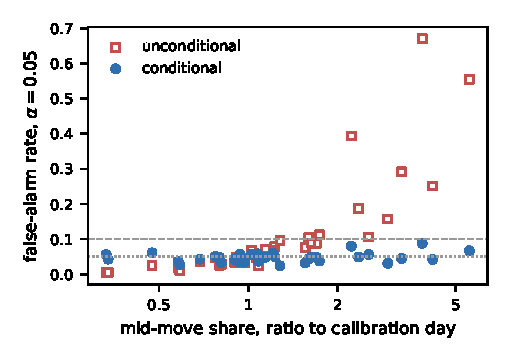
\includegraphics[width=\columnwidth]{figures/fig_jump.pdf}
\caption{Test days, exploratory: each symbol-day's realised false-alarm rate at $\alpha=0.05$ against the ratio of
its mid-move share to that of its calibration day (log scale). Dotted: nominal 0.05; dashed: the rule's limit
0.10.}
\label{fig:jump}
\end{figure}

% =====================================================================================================
\section{Discussion}

\textbf{What the conditional null buys.} Holding the statistics, the combination and the calibration fixed,
replacing a pooled reference set by simulations from the window's own context raised power against all three
footprints. Q1 shows that the gain is in the ranking, not in a looser threshold: at matched size and in the
threshold-free AUC, the conditional detector separates injected from clean copies better. The gain is largest
for spoofing and momentum ignition, whose footprints (a large same-price queue jump, fast mid moves) are large or
small only relative to the current state of the book. Quote stuffing is hard for both detectors (AUC
\aucGenStuff{} and \aucUncStuff), which says more about the panel than about the null: one-lot flickers of a
best queue barely move any statistic in Table~\ref{tab:stats}. The test days support this reading for spoofing
and stuffing, where the conditional detector kept the higher AUC and the higher size-matched power, also with symbols treated as
replicates, but not for ignition: there its AUC and raw power were lower, and its size-matched power was no
different. Because the run failed on validity, the rule confirms the gain for no family.

\textbf{Where it is weak.} The advantage thins in the far tail. At size-matched $\alpha=0.01$ the conditional
detector falls behind for spoofing and stuffing. Its p-values cannot go below $1/(M+1)$, and only windows that
reach the floor get \Mrefine{} continuations, while the unconditional detector always compares with \nRef{}
reference windows. On the test days it was behind in all three families at $\alpha=0.01$ and made almost no
Benjamini--Hochberg discoveries. More continuations would help at linear cost: Stage~0 already took
\hoursLo--\hoursHi{} hours per symbol on a cluster node.

\textbf{Exchangeability is a property of the whole pipeline.} Conformal validity needs calibration and evaluation
windows to be scored by the same procedure. Our refinement rule satisfied this on paper and broke it in practice,
because a clean window's resolution depended on its injected siblings. Any adaptive step in scoring (extra
simulation, early stopping, cached neighbours) must depend only on the window being scored. The drift result
makes a second point: a single calibration day is a fragile reference even for a model that conditions on
context, because the generator's errors change from day to day. Day-before calibration is the simplest fix, and
on the test days it was enough for the conditional detector but not for the unconditional one, which exceeded
the limit on SOL and DOGE. The exploratory analysis of Section~\ref{sec:testresults} points to why: the
unconditional false alarms came on days when the market became much busier than the day before, and conditioning
on the window's context absorbed that change (Fig.~\ref{fig:jump}). This is one run on six symbols, and the
analysis was not planned, so it is a hypothesis for the next pre-registered run rather than a finding. Weighted conformal methods~\cite{tibshirani2019conformal,barber2023conformal} and online adjustment of the
level~\cite{gibbs2021adaptive} are principled alternatives that we have not tried.

\textbf{Operational cost.} Rolling calibration assumes that yesterday was clean. Manipulated windows in the
calibration set raise calibration scores and so make the test conservative rather than liberal. The price is
lost power, not false alarms.

\section{Limitations}
\begin{itemize}
\item \textbf{One confirmatory run.} The design was built on validation days and tested once, on six test days.
That run was not a confirmation, and the reasons it gives (unconditional false alarms, the ignition reversal)
rest on six symbols and six days. Its bootstrap ignores variation between symbols; with symbols resampled
too, the raw power differences for spoofing and stuffing are not distinguishable from zero. The analyses that
explain the outcome were added after it.
\item \textbf{Synthetic labels.} Injected footprints are a stand-in for manipulation. Power against real
manipulation is unknown, and the study detects no real case.
\item \textbf{Passive injection.} The market does not react to the injected orders. A real spoofer's effect on
other traders is not modelled.
\item \textbf{Level 1 only.} Layering at depth and schemes that span venues are invisible here.
\item \textbf{Repair chosen on the same data.} The follow-up rule was written after the Stage-0 result was
known, and its repaired design was selected on the validation days it is evaluated on. On the test days the
conditional detector's false-alarm control held, but the comparison as a whole was not confirmed.
\item \textbf{One month, six symbols, one test-day seed.} The comparison rests on February 2024 crypto futures.
Two further injection seeds left the validation result unchanged (Table~\ref{tab:seeds}), but the test days were
run under one seed.
\end{itemize}

\section{Conclusion}
A fitted order book generator can serve as the null of a surveillance test. On validation days of six crypto
futures contracts, conditioning the null on each window's context raised power against three injected
footprints under the same conformal calibration, and the gain survived matching the false-alarm rate at
$\alpha=0.05$. The pre-registered comparison still failed, on validity: a refinement rule that looked at injected
copies and a single calibration day made the conditional detector flag clean windows too often. Matching the
refinement and calibrating on the day before keeps every symbol within the limit and keeps the power advantage,
under each of three injection seeds.
That repair was found on the same validation days on which it is judged, so we ran it once on six unread test
days under a rule committed beforehand. The result was NOT CONFIRMED. The conditional detector stayed
within the false-alarm limit on every symbol and day; the unconditional one did not, and the rule required both. Power was
higher for spoofing and stuffing and lower for ignition, and the conditional detector stays weak at small
$\alpha$. On these test days a generator-conditional null kept its false-alarm rate within the limit under day-to-day
drift where a pooled null did not;
that it is also more powerful holds at matched false-alarm rates for two of three footprints across symbols,
in an analysis added after the run, and is not confirmed.

\section*{Acknowledgment}
The author thanks Sardar Vallabhbhai National Institute of Technology (SVNIT), Surat, for access to its
high-performance computing cluster.

\section*{Declaration of AI use}
The author used Claude (Anthropic), an AI assistant, to help write and test the analysis code, to check the
references and to help draft and edit the text. The author reviewed and edited the content and takes full
responsibility for it.

% =====================================================================================================
\hbadness=10000
\begin{thebibliography}{99}

\bibitem{vovk2005algorithmic} V.~Vovk, A.~Gammerman, and G.~Shafer, \emph{Algorithmic Learning in a Random
World}. New York, NY, USA: Springer, 2005.

\bibitem{bates2023testing} S.~Bates, E.~Cand\`es, L.~Lei, Y.~Romano, and M.~Sesia, ``Testing for outliers with
conformal p-values,'' \emph{Ann. Statist.}, vol.~51, no.~1, pp.~149--178, 2023.

\bibitem{khatib2026noise} A.~Khatib, ``Noise models matter more than dynamics in synthetic level-1 order flow,''
preprint, 2026. [Online]. Available: \url{https://github.com/Arshad-13/orderflow-noise-models}

\bibitem{putnins2012market} T.~J.~Putni\c{n}\v{s}, ``Market manipulation: A survey,'' \emph{J. Econ. Surveys},
vol.~26, no.~5, pp.~952--967, 2012.

\bibitem{cartea2020spoofing} \'A.~Cartea, S.~Jaimungal, and Y.~Wang, ``Spoofing and price manipulation in
order-driven markets,'' \emph{Appl. Math. Finance}, vol.~27, no.~1--2, pp.~67--98, 2020.

\bibitem{lee2013microstructure} E.~J.~Lee, K.~S.~Eom, and K.~S.~Park, ``Microstructure-based manipulation:
Strategic behavior and performance of spoofing traders,'' \emph{J. Financial Markets}, vol.~16, no.~2,
pp.~227--252, 2013.

\bibitem{wang2017spoofing} X.~Wang and M.~P.~Wellman, ``Spoofing the limit order book: An agent-based model,'' in
\emph{Proc. 16th Int. Conf. Autonomous Agents and Multiagent Systems (AAMAS)}, 2017.

\bibitem{egginton2016quote} J.~F.~Egginton, B.~F.~Van~Ness, and R.~A.~Van~Ness, ``Quote stuffing,''
\emph{Financial Management}, vol.~45, no.~3, pp.~583--608, 2016.

\bibitem{cao2015adaptive} Y.~Cao, Y.~Li, S.~Coleman, A.~Belatreche, and T.~M.~McGinnity, ``Adaptive hidden
Markov model with anomaly states for price manipulation detection,'' \emph{IEEE Trans. Neural Netw. Learn.
Syst.}, vol.~26, no.~2, pp.~318--330, 2015.

\bibitem{tao2022detecting} X.~Tao, A.~Day, L.~Ling, and S.~Drapeau, ``On detecting spoofing strategies in
high-frequency trading,'' \emph{Quant. Finance}, vol.~22, no.~8, pp.~1405--1425, 2022.

\bibitem{kularatnam2024detecting} K.~Kularatnam and T.~Stathaki, ``Detecting and triaging spoofing using temporal
convolutional networks,'' arXiv:2403.13429, 2024.

\bibitem{lin2025detecting} Y.~Lin and P.~Yang, ``Detecting multilevel manipulation from limit order book via
cascaded contrastive representation learning,'' arXiv:2508.17086, 2025.

\bibitem{fabre2025learning} T.~Fabre and D.~Challet, ``Learning the spoofability of limit order books with
interpretable probabilistic neural networks,'' arXiv:2504.15908, 2025.

\bibitem{tiwari2021machine} S.~Tiwari, H.~Ramampiaro, and H.~Langseth, ``Machine learning in financial market
surveillance: A survey,'' \emph{IEEE Access}, vol.~9, pp.~159734--159754, 2021.

\bibitem{coletta2021towards} A.~Coletta, M.~Prata, M.~Conti, E.~Mercanti, N.~Bartolini, A.~Moulin, S.~Vyetrenko,
and T.~Balch, ``Towards realistic market simulations: A generative adversarial networks approach,'' in
\emph{Proc. 2nd ACM Int. Conf. AI in Finance (ICAIF)}, 2021, pp.~1--9.

\bibitem{coletta2023conditional} A.~Coletta, J.~Jerome, R.~Savani, and S.~Vyetrenko, ``Conditional generators for
limit order book environments: Explainability, challenges, and robustness,'' in \emph{Proc. 4th ACM Int. Conf.
AI in Finance (ICAIF)}, 2023, pp.~27--35.

\bibitem{benjamini1995controlling} Y.~Benjamini and Y.~Hochberg, ``Controlling the false discovery rate: A
practical and powerful approach to multiple testing,'' \emph{J. R. Stat. Soc. B}, vol.~57, no.~1, pp.~289--300,
1995.

\bibitem{tibshirani2019conformal} R.~J.~Tibshirani, R.~Foygel~Barber, E.~Cand\`es, and A.~Ramdas, ``Conformal
prediction under covariate shift,'' in \emph{Advances in Neural Information Processing Systems 32}, 2019.

\bibitem{barber2023conformal} R.~Foygel~Barber, E.~J.~Cand\`es, A.~Ramdas, and R.~J.~Tibshirani, ``Conformal
prediction beyond exchangeability,'' \emph{Ann. Statist.}, vol.~51, no.~2, pp.~816--845, 2023.

\bibitem{gibbs2021adaptive} I.~Gibbs and E.~Cand\`es, ``Adaptive conformal inference under distribution shift,''
in \emph{Advances in Neural Information Processing Systems 34}, 2021.

\bibitem{liu2020cauchy} Y.~Liu and J.~Xie, ``Cauchy combination test: A powerful test with analytic p-value
calculation under arbitrary dependency structures,'' \emph{J. Amer. Statist. Assoc.}, vol.~115, no.~529,
pp.~393--402, 2020.

\bibitem{phipson2010permutation} B.~Phipson and G.~K.~Smyth, ``Permutation p-values should never be zero:
Calculating exact p-values when permutations are randomly drawn,'' \emph{Stat. Appl. Genet. Mol. Biol.},
vol.~9, no.~1, Art.~39, 2010.

\end{thebibliography}

\end{document}
